\chapter{Model Development}
\label{chap:model}

% ============================================================================
% CHAPTER PURPOSE -- VERY HIGH PRIORITY / TECHNICAL CORE
% Construct the undercut analysis methodology from the engineering question to
% the final cumulative scenario comparison. The reader should understand what
% is compared, over which interval, and why each model term is required before
% encountering the fully indexed formulation.
%
% Narrative order:
% race state -> terminology -> scenarios -> comparison window -> lap time
% prediction -> model extensions -> cumulative comparison -> decision metrics.
% ============================================================================

\section{Modelling Approach}
\label{sec:modelling-approach}

% Keep this opening conceptual. Detailed equations begin only after the reader
% understands the two hypothetical futures and their common time window.

The model evaluates whether an attacking driver would gain or lose time by
making a pit stop at a selected point in a historic race. It is deterministic:
the same reference race state and parameter values always produce the same
result. It is also comparative rather than predictive of the complete race.
Two hypothetical futures are generated from one decision point and evaluated
over a common time interval:

\begin{itemize}
    \item In the \emph{stay out scenario}, the attacking driver remains on the
    current tyre at the decision point.
    \item In the \emph{undercut scenario}, the attacking driver pits at the
    decision point and continues on the specified replacement tyre.
\end{itemize}

The target driver's assumed behaviour is common to both scenarios. This
isolates the effect of the attacking driver's decision rather than attributing
the result to an abnormal stop or an unrelated change in the target driver's
pace. Lap times are predicted individually and accumulated over a defined
comparison window. The principal output is a continuous time gain or loss; the
corresponding track-position outcome is reported separately.

The method is intended to capture the dominant tyre-driven mechanism of an
undercut while remaining explainable and suitable for sensitivity analysis. It
does not attempt to reproduce the stochastic behaviour of a complete Formula
One race or replace the broader judgement required by a race strategy team.

\section{Reference Race State and Terminology}
\label{sec:reference-race-state}

The calculation begins from a reference race state reconstructed at the chosen
decision point. At minimum, this state identifies the attacking and target
drivers, their relative time gap, current compounds and tyre ages. It also
contains, or provides the data required to derive, the pace parameters used by
the lap time model. Both hypothetical scenarios use the same reference state;
only the attacking driver's pit decision changes.

Table \ref{tab:model_terminology} defines the model-specific terms used
throughout this chapter. These definitions are distinct from the general
Formula One terminology provided in the glossary.

\begin{table}[htbp]
\centering
\caption{Terminology used throughout the proposed undercut model.}
\label{tab:model_terminology}

\begin{tabular}{|P{0.22\textwidth}|P{0.73\textwidth}|}
\hline
\textbf{Term} & \textbf{Definition} \\
\hline

Attacking Driver &
The driver attempting to gain track position by performing an undercut against a competitor. \\
\hline

Target Driver &
The competitor against whom the undercut manoeuvre is evaluated. \\
\hline

Decision Point &
The lap at which the attacking driver is assumed to decide whether to remain on track or enter the pit lane. Both strategy scenarios diverge from this point. \\
\hline

Comparison Window &
The sequence of laps over which the stay out and undercut scenarios are evaluated and compared. \\
\hline

Stay Out Scenario &
The hypothetical strategy in which the attacking driver remains on track at the decision point while all other modelling assumptions remain unchanged. \\
\hline

Undercut Scenario &
The hypothetical strategy in which the attacking driver enters the pit lane at the decision point while all other modelling assumptions remain unchanged. \\
\hline

Reference Race State &
The observed state of the historic race at the decision point, including the selected drivers, tyre compounds, tyre ages and time gap, from which the hypothetical strategy scenarios are generated. \\
\hline

\end{tabular}
\end{table}

\section{Strategy Scenarios}
\label{sec:scenario-definition}

% MUST-HAVE FIGURE:
% Add a parallel timeline showing the attacking and target drivers, decision
% point, both attacking-driver alternatives, target stop, offset laps and one
% common comparison endpoint.

\subsection{Decision Point and Driver Roles}
\label{subsec:driver-roles}

The attacking driver is the driver for whom the pit decision is evaluated. The
target driver is the competitor whose track position the attacker is attempting
to gain. The decision point is placed at a defined lap boundary so that tyre
age and lap indexing remain unambiguous. The pre-decision time gap is retained
as an initial condition and is not treated as time created by the undercut.

% TODO: State the exact timing convention used by the implementation. For
% example, define whether the decision occurs at pit entry on the attacker's
% in lap or at the start of the following timing lap. Use the same convention
% in Chapter \ref{chap:implementation} and all validation cases.

\subsection{Stay Out Scenario}
\label{subsec:reference-scenario}

In the stay out scenario, the attacking driver remains on the current tyre at
the decision point. The tyre therefore continues to age during the offset
period. This scenario represents the reference against which the earlier stop
is evaluated; it is not a claim that remaining on track indefinitely is a
viable strategy.

% TODO: Define the attacker's eventual reference stop timing. It must give the
% two scenarios an equivalent endpoint if common pit loss is to be cancelled
% rather than accidentally omitted.

\subsection{Undercut Scenario}
\label{subsec:undercut-scenario}

In the undercut scenario, the attacking driver enters the pit lane at the
decision point and begins the offset period on the specified replacement tyre.
Its starting age may be zero for a new set or greater than zero for a used set.
The first post-stop laps may also include warm up and traffic penalties if
those extensions are enabled.

\section{Comparison Window}
\label{sec:comparison-window}

The comparison window is the common interval over which the two hypothetical
futures are evaluated. It begins at the decision point and includes the laps
during which the attacking driver's tyre state differs between the scenarios.
It ends at an equivalent race state after the reference stop has been accounted
for in both scenarios. If the target is expected to stop $n$ laps after the
attacker's decision, $n$ defines the offset being evaluated.

Comparing cumulative time over this window is essential. One quick lap on a
fresh tyre does not establish whether a pit stop decision is advantageous; the
relevant quantity is the total time gained or lost before the scenarios return
to a comparable state.

% TODO -- MUST RESOLVE BEFORE VALIDATION:
% - define whether in laps and out laps are complete observed/modelled laps;
% - state whether the endpoint is target pit exit or completion of its out lap;
% - state how offsets of one, two, three, ... laps are enumerated;
% - ensure the implementation uses the same boundaries.

\subsection{Pit Lane Loss and Symmetry}
\label{sec:pit-loss}

Pit lane traversal and service time do not generate the undercut advantage. If
both scenarios contain an equivalent pit stop and are evaluated at the same
post-stop state, their common pit lane loss cancels. For a common pit loss
$P$, the difference between cumulative scenario times is

\begin{equation}
\begin{split}
\Delta T(n)
&= \left(T_{\mathrm{stay,laps}}(n)+P\right)
 - \left(T_{\mathrm{undercut,laps}}(n)+P\right) \\
&= T_{\mathrm{stay,laps}}(n)-T_{\mathrm{undercut,laps}}(n).
\end{split}
\label{eq:pit-loss-cancellation}
\end{equation}
\myequation{Cancellation of common pit lane loss}

The undercut gain is therefore produced principally by relative lap time
performance during the offset period. Pit lane loss remains necessary when
determining the attacker's immediate rejoin position and consequent traffic
exposure. It must also be retained if the model deliberately represents unequal
stops. A slow target stop is treated as an observed anomaly, not as a mechanism
on which an undercut decision should rely.

\section{Model Architecture and Information Flow}
\label{subsec:model-architecture}

Figure \ref{fig:architecture-model} summarises the information flow from the
historic reference state to the engineering outputs. The lap time model is one
component of the method: it supplies predictions to the parallel scenario
calculations, which are then accumulated and compared.

% TODO: Review the figure once the final model terms and scenario engine are
% fixed. Required flow:
% Historic race data -> reference race state -> lap time model -> stay out and
% undercut scenarios -> cumulative comparison -> decision metrics.

\begin{figure}[htbp]
    \centering
    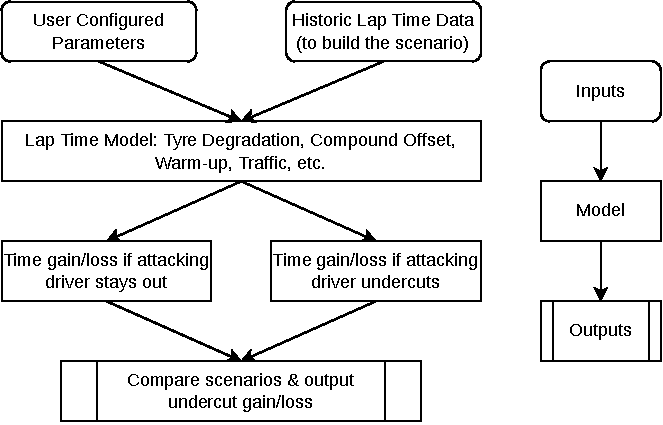
\includegraphics[width=\textwidth]{Figures/3_architecture_model.pdf}
    \caption{Information flow through the proposed undercut analysis model.}
    \label{fig:architecture-model}
\end{figure}

\section{Lap Time Model}
\label{sec:lap-time-model}

The scenario comparison requires a predicted lap time for each driver state.
The lap time model is therefore a supporting component rather than the sole
contribution of the dissertation. It is introduced in a deliberately simple
form before effects that require additional terms are added.

\subsection{Minimum Model}
\label{subsec:minimum-model}

The minimum model assumes that lap time $L$ is determined by reference pace
$B$, a compound offset $C$, and degradation loss $D(a)$ at tyre age $a$:

\begin{equation}
L=B+C+D(a).
\label{eq:minimum-lap-time}
\end{equation}
\myequation{Minimum lap time model}

Indices are intentionally omitted from \cref{eq:minimum-lap-time}. At this
stage they would add notation without improving the physical explanation. The
driver, scenario and lap indices are introduced only when the two futures are
accumulated in \cref{sec:cumulative-formulation}.

\subsubsection{Reference Pace}

The reference pace represents the underlying lap time of the selected driver
and car after the modelled tyre effects have been separated. When a common
event reference is used, an individual pace adjustment $P_d$ may be applied:

\begin{equation}
B_d=B_{\mathrm{ref}}+P_d.
\label{eq:driver-specific-ref-time}
\end{equation}
\myequation{Driver-specific reference pace}

% TODO: Choose one final estimation method. State the laps used, excluded lap
% types, fuel or track-evolution correction, and whether P_d is derived from
% historic data or supplied as an input. The method must prevent genuine
% driver/car pace from being misidentified as a tyre effect.

\subsubsection{Compound Offset}

The compound offset $C$ represents the lap time difference associated with a
tyre compound relative to a declared reference compound. As discussed in
\cref{subsec:tyre-compounds} and illustrated in
\cref{fig:1_conceptual_tyres}, the compounds provide different levels of grip
and durability. The offset is event-specific unless validation establishes
that a more general value is defensible.

% TODO: State how offsets are derived or supplied. Do not use generic fixed
% Soft/Medium/Hard values as evidence; label worked-example values as
% illustrative.

\subsubsection{Linear Degradation}

For the minimum model, degradation is approximated as a linear loss over the
short comparison window:

\begin{equation}
D(a)=ka,
\label{eq:linear-degradation}
\end{equation}

where $k$ is the degradation rate in seconds per lap of tyre age. Substitution
into \cref{eq:minimum-lap-time} gives

\begin{equation}
L=B+C+ka.
\label{eq:model-plus-tyre-degradation}
\end{equation}
\myequation{Minimum lap time model with linear degradation}

The approximation does not imply that an entire tyre stint is physically
linear. It provides an interpretable local model whose adequacy over the short
offset window can be tested against historic cases and through sensitivity
analysis.

% TODO: Define tyre age precisely. State whether age zero denotes an unused
% tyre before its out lap or the first completed timed lap. This convention is
% a likely source of off-by-one implementation errors.

\section{Progressive Model Extensions}
\label{sec:model-extensions}

Reference pace, compound offset and linear degradation specify terms already
present in the minimum model. The following additions are genuine extensions:
each introduces an effect that the minimum formulation cannot represent. For
every retained extension, document its engineering motivation, mathematical
form, parameter source and validation status.

\subsection{Tyre Warm Up Loss}
\label{subsec:warmup-model}

Freshly fitted tyres may not deliver their steady-state performance immediately.
A warm up term $W(i)$ is therefore added, where $i$ is the post-stop lap index:

\begin{equation}
L=B+C+D(a)+W(i).
\label{eq:model-plus-warmup}
\end{equation}
\myequation{Lap time model with tyre warm up loss}

% TODO: Select and justify the implemented form of W(i). If the software uses
% one out-lap penalty, state that directly. Do not imply a thermal tyre model.

\subsection{Traffic and Rejoin Effects}
\label{subsec:traffic-model}

An early stop can cause the attacking driver to rejoin behind slower traffic.
This changes the achievable lap time even when the fresh tyre advantage is
large. A traffic or rejoin penalty $R(i)$ extends the model to

\begin{equation}
L=B+C+D(a)+W(i)+R(i).
\label{eq:model-plus-traffic}
\end{equation}
\myequation{Lap time model with warm up and traffic effects}

Rejoin feasibility and time loss are related but distinct. Pit lane loss and
the current race gaps determine where the car rejoins; $R(i)$ represents the
additional lap time consequence after it has rejoined.

% TODO: State whether R(i) is derived from historic positions and gaps, entered
% as a configurable penalty, or omitted from the validated model. Do not claim
% predictive traffic simulation unless it has been implemented and verified.

\subsection{Used Replacement Tyres}
\label{subsec:used-tyres}

A replacement set need not be new. A used set is represented by assigning a
non-zero initial tyre age in the undercut scenario. This changes the degradation
term without requiring another additive lap time component. Any interaction
with the selected warm up representation must be stated explicitly.

\subsection{Effects Outside the Retained Model}
\label{subsec:optional-effects}

% LOWER PRIORITY: discuss only effects relevant to the final implementation.
% Candidate omissions include fuel mass, track evolution, non-linear
% degradation, driver variability and stochastic race interruptions. Explain
% the capability each would add before proposing it as future work.

\section{Cumulative Scenario Formulation}
\label{sec:cumulative-formulation}

Once the lap time components have been established, indices are required to
distinguish driver $d$, scenario $s$ and lap $i$. The complete retained lap time
model is written as

\begin{equation}
L_{d,s}(i)=B_d+C_{c_{d,s,i}}+D_{c_{d,s,i}}(a_{d,s,i})
            +W_{c_{d,s,i}}(i)+R_d(i).
\label{eq:complete-lap-time-model}
\end{equation}
\myequation{Complete indexed lap time model}

% Remove terms from this equation if they are not present in the final tested
% implementation, or mark them explicitly as optional. The dissertation must
% describe the model actually evaluated rather than an aspirational model.

The cumulative predicted time for scenario $s$ over $n$ comparison laps is

\begin{equation}
T_s(n)=\sum_{i=1}^{n}L_{\mathrm{att},s}(i)+Q_s,
\label{eq:cumulative-scenario-time}
\end{equation}
\myequation{Cumulative scenario time}

where $Q_s$ contains only scenario-specific pit, in-lap, out-lap or rejoin
adjustments not already included in the lap predictions. Common terms must not
be counted twice. The predicted undercut gain is defined as

\begin{equation}
G(n)=T_{\mathrm{stay}}(n)-T_{\mathrm{undercut}}(n).
\label{eq:undercut-gain}
\end{equation}
\myequation{Predicted undercut gain}

Under this sign convention, $G(n)>0$ indicates that pitting at the decision
point is predicted to save time, while $G(n)<0$ indicates a predicted loss.
This convention must be used consistently in the software, plots and validation
results.

\section{Model Outputs and Decision Metrics}
\label{sec:model-outputs}

The cumulative strategy gain $G(n)$ is the primary engineering output. Applying
that gain to the observed pre-decision gap produces a predicted post-stop gap
to the target driver. A track-position indicator can then report whether the
predicted gap crosses zero, while retaining the underlying continuous result
for interpretation and sensitivity analysis.

% TODO: Define the initial-gap sign convention and give the exact post-stop-gap
% equation. Also state whether the software reports the best tested offset,
% crossover lap, rejoin traffic warning, or any uncertainty interval.

\section{Definitions and Notation}
\label{subsec:notation}

Table \ref{tab:model_notation} consolidates the symbols introduced throughout
the model. A symbol is explained in detail when it first adds a capability; the
table then provides a single reference for its unit and scope.

\begin{table}[htbp]
\centering
\caption{Notation used throughout the proposed undercut model.}
\label{tab:model_notation}

\begin{tabular}{|l|l|p{7.5cm}|l|}
\hline
\textbf{Symbol} & \textbf{Unit} & \textbf{Definition} & \textbf{Scope} \\
\hline

$i$ & -- &
Lap index within the comparison window. &
$i = 1,2,\ldots,n$ \\
\hline

$n$ & laps &
Number of laps included in the comparison window. &
Scenario-independent \\
\hline

$a$ & laps &
Tyre age at the start of a lap. &
Driver-specific \\
\hline

$d$ & -- &
Driver identifier. &
Attacking or target driver \\
\hline

$c$ & -- &
Tyre compound identifier. &
Soft, Medium or Hard \\
\hline

$s$ & -- &
Strategy scenario. &
Undercut or Stay Out \\
\hline

$B_d$ & s &
Reference lap time of driver $d$, excluding tyre-related effects and configurable model adjustments. &
Driver \\
\hline

$P_d$ & s &
Pace adjustment of driver $d$ relative to the event reference pace. &
Driver \\
\hline

$C_c$ & s &
Lap time offset associated with tyre compound $c$. &
Compound \\
\hline

$D_c(a)$ & s &
Lap time loss due to tyre degradation as a function of tyre age. &
Compound, tyre age \\
\hline

$W_c(i)$ & s &
Warm-up penalty applied following a tyre change. &
Compound, lap \\
\hline

$R_d(i)$ & s &
Additional configurable lap time penalty due to traffic or other external effects. &
Driver, lap \\
\hline

$L_{d,s}(i)$ & s &
Predicted lap time of driver $d$ on lap $i$ under strategy scenario $s$. &
Driver, scenario, lap \\
\hline

$P$ & s &
Pit lane traversal and service loss common to equivalent stops. &
Pit stop \\
\hline

$Q_s$ & s &
Scenario-specific timing adjustments not already included in the predicted lap times. &
Scenario \\
\hline

$T_s(n)$ & s &
Cumulative predicted race time after $n$ comparison laps for strategy scenario $s$. &
Scenario \\
\hline

$G(n)$ & s &
Predicted undercut gain, defined as stay out scenario time minus undercut scenario time. &
Comparison window \\
\hline

\end{tabular}
\end{table}


\section{Model Parameters and Data Provenance}
\label{sec:model-parameters}

% VERY HIGH PRIORITY. Add one or more readable tables with:
% Parameter | Symbol | Unit | Scenario/driver | Source | Treatment.
% Separate measured historic fields, values derived from those fields, and
% configurable assumptions. Naming an API alone is not sufficient provenance.
% Resolve FastF1 versus OpenF1 consistently across Chapters 3--5, references,
% and the data/licensing appendix.
%
% Identify the baseline value and sensitivity range for every parameter tested
% in Chapters \ref{chap:validation-method} and \ref{chap:results}.

\section{Worked Numerical Example}
\label{sec:worked-example}

% HIGH VALUE. Add a deliberately simple fictional example containing:
% - the initial gap and both drivers' tyre states;
% - two or three offset laps;
% - the stay out and undercut lap predictions;
% - cumulative totals and common pit-loss cancellation;
% - G(n), the post-stop gap and the decision interpretation.
% Label every value as illustrative rather than validation evidence.

\section{Assumptions and Applicability}
\label{sec:model-assumptions}

% Add a table: Assumption | Rationale | Consequence | Tested/mitigated in.
% Include deterministic inputs, local linear degradation, short comparison
% window, equivalent pit losses, dry/green running, two-driver scope, baseline
% pace treatment, traffic representation and data completeness.
%
% An assumption defines model operation. A limitation is the resulting
% restriction on applicability or generalisability. Keep those ideas distinct.

\section{Chapter Summary}
\label{sec:model-summary}

% Summarise only the final retained model, output metrics and principal
% assumptions. Conclude by stating that Chapter \ref{chap:implementation}
% translates the methodology into software without changing its engineering
% logic.
